\section{Tecniche di predizione dei salti}\label{capitolo2}
Come abbiamo visto nel \chaptername\,\ref{capitolo1} i branch condizionati sono istruzioni di salto che vengono eseguite soltanto se viene soddisfatta la condizione. L'indirizzo di destinazione del branch viene sostituito nel program counter al posto dell'indirizzo dell'istruzione sequenziale successiva.
Nel caso di ambiente MIPS possiamo distinguere due tipi di branch:
\begin{itemize}
\item \texttt{beq}: \emph{branch on equal} che richiede che i valori nei registri da confrontare siano uguali.
\item \texttt{bne}: \emph{branch on not equal} che richiede che i valori nei registri da confrontare siano diversi.
\end{itemize}
Come abbiamo visto nel capitolo precedente le istruzioni di salto condizionato sono nel formato \emph{I-Format} e un'istruzione di questo tipo è suddivisa nei diversi campi come mostrato in \figurename\,\ref{fig:branch}
\begin{figure}
\centering
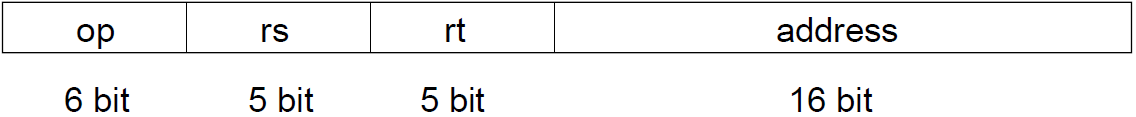
\includegraphics[scale=0.5]{img/condbranch.png}
\caption{Esempio di istruzione di branch}\label{fig:branch}
\end{figure}
Dove il campo \texttt{address} indica l'indirizzo relativo rispetto al program counter che punta all'etichetta di salto.\\
Questo tipo di istruzione sfrutta solo quattro dei cinque stadi della pipeline come mostrato in \figurename\,\ref{fig:branchpipe}; durante l'instruction fetch si recupera l'istruzione da eseguire e si aggiorna il program counter all'istruzione sequenziale successiva, successivamente durante la fase di instruction decode si leggono i due registri da comparare. Durante la fase di \emph{execution} la ALU compara i due registri e calcola il valore di destinazione del salto. Durante la fase \emph{Memory Access} si decide in base al valore della comparazione effettuata dalla ALU se aggiornare il PC con il valore del salto.
\begin{figure}
\centering
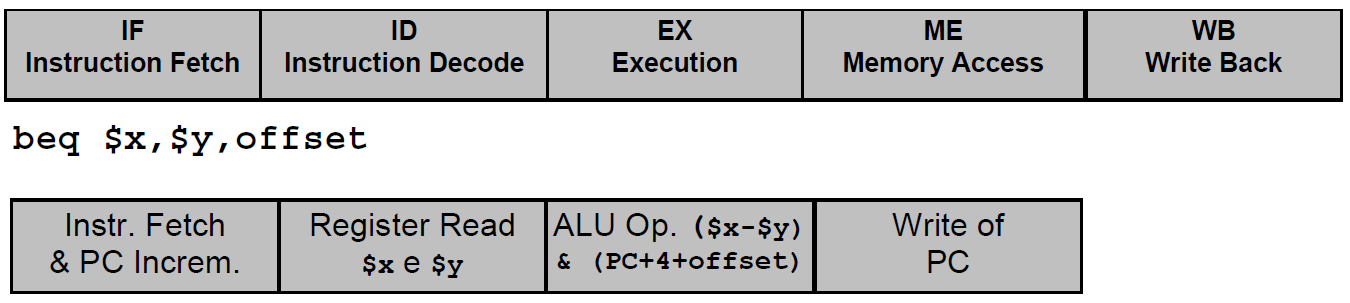
\includegraphics[scale=0.5]{img/branchpipe.png}
\caption{Suddivisione dell'esecuzione di un'istruzione di salto nelle varie fasi di una pipe}\label{fig:branchpipe}
\end{figure}
\subsection{Il problema del Control Hazard}
Il \emph{control hazard} è il problema di decidere quale istruzione eseguire prima che la condizione di salto sia valutata. I problemi di \emph{control hazard} nascono ogni qualvolta nella pipeline sia necessario modificare il valore del PC. Tali problemi riducono perciò la velocità della pipeline riducendo lo speedup ideale a causa di introduzioni di stalli nella pipeline.\\
Per alimentare la pipeline è necessario prelevare una nuova istruzione ad ogni ciclo di clock ma la decisione se effettuare o non effettuare un salto avviene solo durante lo stage \emph{MEM}. Questo ritardo nel determinare l'istruzione successiva corretta è chiamato \emph{Control Hazard} o \emph{Conditional Branch Hazard}.\\
Analizziamo ora l'esempio di \figurename\,\ref{fig:branchexe} in questo esempio la prima istruzione è un salto condizionato che viene valutato solo nella fase si MEM; durante l'esecuzione di tale istruzione vengono prelevate anche le tre istruzioni successive per continuare ad alimentare la pipeline. Se il salto non viene eseguito l'esecuzione è corretta e può proseguire, nel caso in cui, invece, il salto venga eseguito allora diventa necessario effettuare il \emph{flush} delle tre istruzioni prelevate durante l'esecuzione del branch.
\begin{figure}
\centering
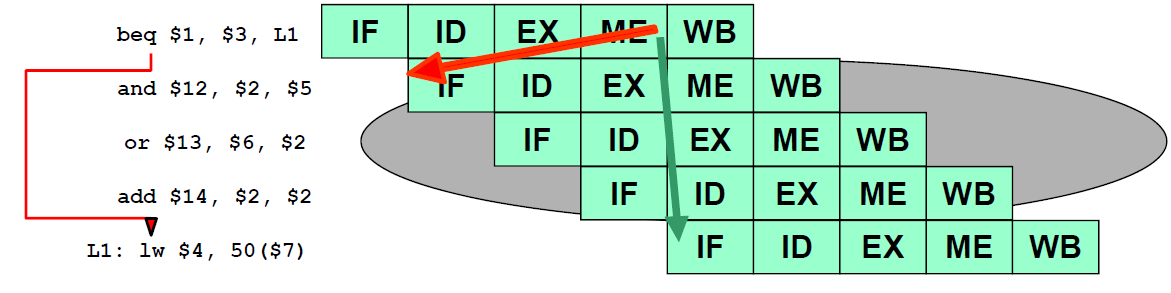
\includegraphics[scale=0.5]{img/branchexe.png}
\caption{Esempio di esecuzione di un istruzione di salto}\label{fig:branchexe}
\end{figure}
Una possibile soluzione al problema è quella di attendere la decisione del salto prima di effettuare qualsiasi altra operazione; questo comporta l'inserimento di "stalli" nella pipeline; più precisamente sono necessari:
\begin{itemize}
\item tre stalli senza forwarding
\item due stalli con forwarding
\end{itemize}
Nel caso in cui il salto non venga eseguito, tuttavia, la penalità di tre cicli   di stallo non è giustificata. Un'altra soluzione è quella di assumere che il salto non sia mai eseguito e quindi scartare le tre istruzioni nel caso in cui il salto venga preso.\\
Una terza soluzione è quella di aggiungere delle risorse hardware per permettere di:
\begin{itemize}
\item comparare i registri
\item calcolare l'indirizzo di destinazione del branch
\item aggiornare il valore del PC
\end{itemize}
il prima possibile nella catena della pipeline.
Nei processori MIPS tutto questo avviene durante lo stage ID come mostrato in \figurename\,\ref{fig:hwbranch}
\begin{figure}
\centering
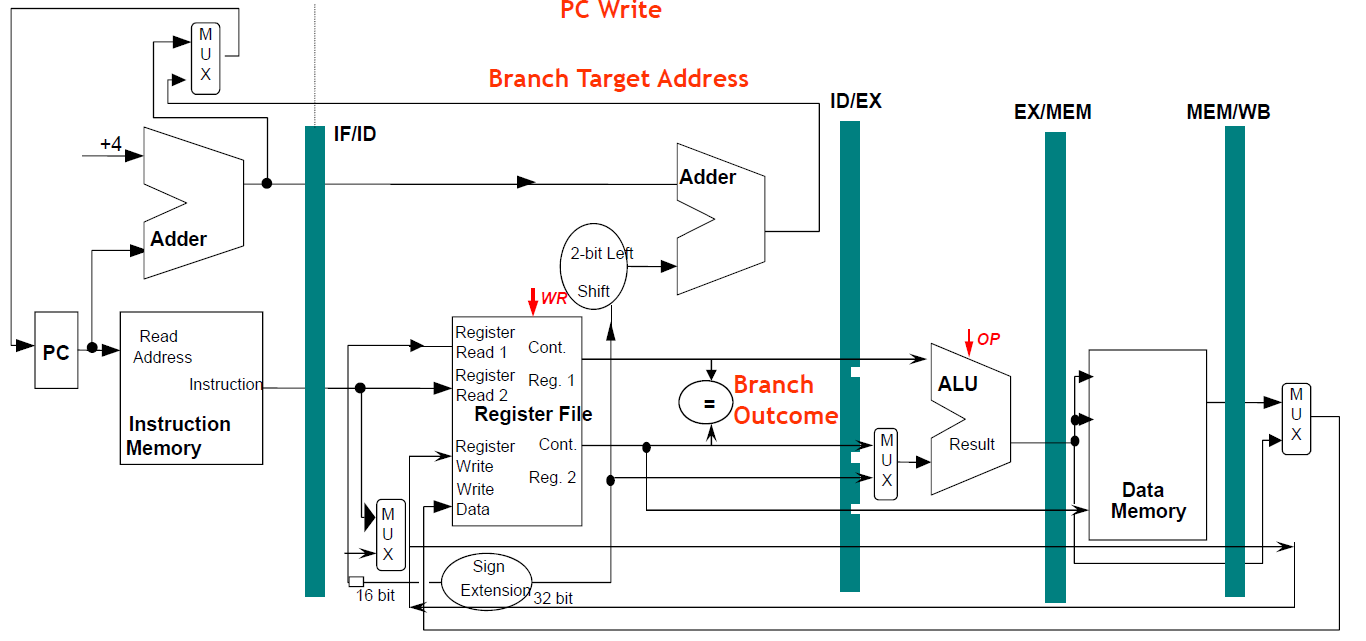
\includegraphics[scale=0.4,angle=90]{img/hwbranch.png}
\caption{Hardware aggiuntivo per risolvere i problemi di controllo}\label{fig:hwbranch}
\end{figure}
Utilizzando queste tecniche si riesce a ridurre al minimo il costo per recuperare la corretta esecuzione di un branch nel caso di scelta sbagliata, riducendo a uno il numero degli stalli da introdurre.\\
Tuttavia queste tecniche comportano tuttavia una riduzione delle performance quantificabile tra il $10\%$ e il $30\%$ in base alla frequenza dei salti.
Tali perdite di performance possono essere ridotte ulteriormente tramite alcune tecniche.
\subsection{Tecniche di predizione dei salti}
In generale il problema dei salti diventa importante quando si tratta di processori con delle pipeline profonde, dove il costo di una predizione errata è molto alto. Lo scopo principale delle tecniche di predizione dei salti è quello di predire il prima possibile il risultato di un istruzione di salto.\\
Le performance di una tecnica di predizione si possono misurare in:
\begin{itemize}
\item \textbf{Accuratezza:} misurata in termini di percentuale di predizioni sbagliate.
\item \textbf{Costo:} misurato come tempo perso nel caso di predizione sbagliata.
\end{itemize}
Le tecniche di predizione dei salti possono essere suddivise in due categorie:
\begin{itemize}
\item \emph{Tecniche di predizione statiche:} le azioni intraprese per il branch sono prefissate e uguali per tutta l'esecuzione e determinate a tempo di compilazione.
\item \emph{Tecniche di predizione dinamiche:} in questo caso le decisioni variano a seconda dell'esecuzione.
\end{itemize}
\subsubsection{Tecniche di predizione statiche}
Le tecniche di predizione statiche sono utilizzate soprattutto in quei processi dove ci si aspetta che i salti siano altamente predicibili. Alcune tecniche statiche di predizione dei salti sono:
\begin{itemize}
\item Branch Always Not Taken (Predicted-Not-Taken)
\item Branch Always Taken (Predicted-Taken)
\item Backward Taken Forward Not Taken (BTFNT)
\item Profile-Driven Prediction
\item Delayed Branch
\end{itemize}
\paragraph{Branch Always Not Taken}
In questa particolare tecnica assumiamo che il salto non venga mai intrapreso e    le istruzioni vengono prelevate sequenzialmente e il flusso prosegue come se il  salto non venga intrapreso. Se la condizione nello stage ID non viene soddisfatta la predizione è corretta e perciò non abbiamo perdita di performance.\\
Se la condizione nello stage ID risulta soddisfatta allora la predizione è errata e il salto viene effettuato. A questo punto dobbiamo effettuare il flush delle successive istruzioni che sono già state messe in esecuzione sostituendole con delle \texttt{nop} e riprendere l'esecuzione inserendo nella pipeline la prima istruzione del salto. Tutto questo porta ad una penalità di un ciclo di clock.
\begin{figure}[htb]
\centering
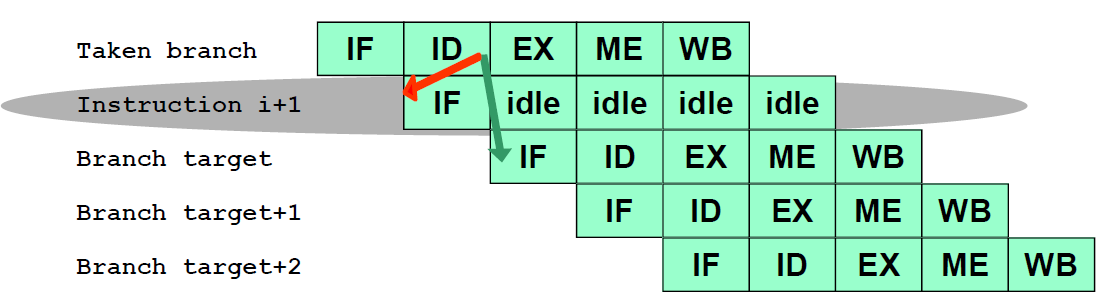
\includegraphics[scale=0.5]{img/branchpenality.png}
\caption{Esempio di penalità dovuto ad una predizione sbagliata}\label{fig:bantpenality}
\end{figure}
\paragraph{Branch Always Taken}
In alternativa al tipo di predizione precedente si può considerare che ogni salto sia sempre eseguito. Ogni qualvolta che un salto è decodificato e il suo indirizzo di destinazione è calcolato allora si assume che il salto sia eseguito e si introducono nella pipeline le istruzioni puntate dall'indirizzo di destinazione. Questo tipo di previsione ha senso in quelle pipeline dove l'indirizzo target è calcolato prima della comparazione dei registri.\\
Nelle pipeline di tipo MIPS noi non conosciamo l'indirizzo di destinazione prima della valutazione delle condizioni di salto così non vi è alcun vantaggio dall'utilizzo di questa tecnica.
\paragraph{Backward Taken Forward Not Taken (BTFNT)}
La predizione di questa tecnica si basa sulla direzione del salto, ovvero se i salti sono all'indietro sono previsti come eseguiti (come ad esempio nei cicli) salti in avanti sono considerati come non eseguiti.
\paragraph{Profile-driven Prediction}
Questo tipo di predizione si basa su dati raccolti da precedenti esecuzioni del programma utilizzando alcune funzioni del compilatore.
\paragraph{Delayed Branch Technique}
In questo tipo di tecnica il compilatore schedula una particolare istruzione indipendente dal salto in un campo chiamato \textbf{branch delay slot}. L'istruzione in questo slot viene eseguita ogni qualvolta che  il salto viene eseguito oppure no. Se assumiamo il ritardo dovuto ad un salto pari ad un ciclo di clock allora gli slot necessari per le istruzioni sono uno.
Un esempio di questa tecnica è mostrato in \figurename\,\ref{fig:branchdelay} dove nel \emph{branch delay slot} viene inserita un'istruzione di \texttt{add} indipendente dal ciclo.
\begin{figure}[htb]
\centering
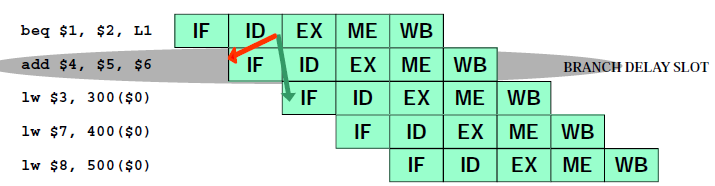
\includegraphics[scale=0.5]{img/branchdelay.png}
\caption{Esempio di utilizzo del branch delay slot}\label{fig:branchdelay}
\end{figure}
Sia nel caso che il salto sia eseguito sia nel caso non sia eseguito l'istruzione dopo quella di salto è sempre quella del \emph{delay slot} tuttavia nel caso il salto sia eseguito dopo l'istruzione del \emph{delay slot} l'esecuzione prosegue con le istruzioni del salto viceversa nel caso non sia eseguito allora l'esecuzione prosegue con le istruzioni successive.\\
Il compilatore deve essere in grado di selezionare l'istruzione da inserire nel delay slot in modo che essa sia valida ed utile. Ci sono quattro modi per selezionare tale istruzione:
\begin{itemize}
\item From Before
\item From Target
\item From Fall-Through
\item From After
\end{itemize}
La tecnica \emph{From Before} prevede di selezionare un istruzione indipendente selezionata tra quelle che precedono il salto in tale modo l'istruzione viene sempre eseguita. Il metodo \emph{From Target} prevede la copia dell'istruzione puntata dal salto; questa tecnica è preferibile quando il salto ha un alta probabilità di essere eseguito. Un esempio di utilizzo di questa tecnica è mostrato in \figurename\,\ref{fig:fromtarget}.
\begin{figure}[htb]
\centering
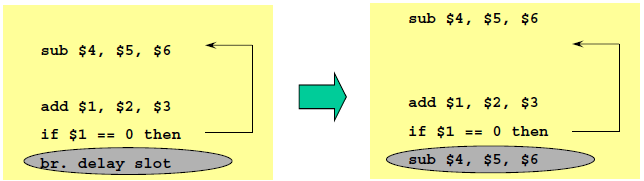
\includegraphics[scale=0.5]{img/fromtarget.png}
\caption{Esempio di selezione dell'istruzione \emph{From Target}}\label{fig:fromtarget}
\end{figure}
La tecnica \emph{From Fall-Through} e contrapposta alla tecnica \emph{From Target} infatti questa prevede che l'istruzione selezionata per il delay slot sia la prima istruzione che verrebbe prelevata nel caso di salto non eseguito come si vede dalla \figurename\,\ref{fig:fromfall}
\begin{figure}[htb]
\centering
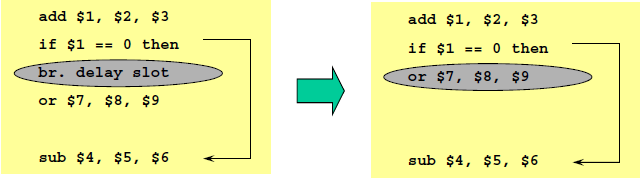
\includegraphics[scale=0.5]{img/fromfall.png}
\caption{Esempio di uso della tecnica \emph{From Fall-Through}}\label{fig:fromfall}
\end{figure}
Questo tipo di tecnica è preferibile quando il salto ha un alta probabilità di essere non eseguito.
Perché le ultime due tecniche risultino corrette è necessario che le istruzioni eseguite quando il salto non prende la direzione prevista risultino ininfluenti rispetto alla normale esecuzione del programma. Questo è possibile ad esempio se l'istruzione nel delay slot agisce su dei registri che sono inutilizzati nel caso di risultato inaspettato del salto.\\
In generale il compilatore è in grado di assegnare il 50\% dei \emph{delay slot} con istruzioni valide e utili, all'altro 50\% viene riempito con istruzioni di tipo \texttt{nop}. Nel caso di pipeline più profonda il tempo necessario per valutare il salto è maggiore di un ciclo di clock e di conseguenza aumenta il numero di delay slot da riempire; diventa sempre più difficile perciò riempire tali slot con istruzioni valide e utili. Le principali limitazioni che nascono sono dovute alle restrizioni sulle istruzioni che possono essere schedulate e sull'abilità del compilatore di predire staticamente il risultato del salto.\\
Per migliorare l'abilità del compilatore di riempire i \emph{delay slot} molti processori hanno introdotto il \textbf{canceling or nullifing branch} ovvero salti nei quali è anche compresa la predizione della direzione del salto. Quando la predizione è verificata allora il contenuto del \emph{delay slot} è eseguito in caso contrario viene eseguita una \texttt{nop}
\subsubsection{Tecniche di predizione dinamiche}
L'idea di base in questo tipo di tecnica è quella di utilizzare il risultato di esecuzioni di salti passate per predire i salti futuri. Possiamo utilizzare dell'hardware per predire dinamicamente il risultato del salto; la predizione dipende dal comportamento dei salti durante l'esecuzione.\\
Il meccanismo di predizione dinamica si basa su due meccanismi che interagiscono tra loro:
\begin{itemize}
\item \textbf{Branch Outcame Predictor:} che tenta di predire la direzione del branch.
\item \textbf{Branch Target Predictor:} che calcola l'indirizzo di destinazione del salto nel caso in cui la condizione del salto abbia un risultato positivo.
\end{itemize}
Questi due moduli sono usate dall'unità di Instruction Fetch per predire la prossima istruzione da prelevare dall'I-Cache. Nel caso in cui il salto non venga eseguito il PC viene semplicemente incrementato, nel caso in cui, invece il branch venga preso il branch target predictor fornisce l'indirizzo di destinazione. Esiste inoltre una tabella chiamata \textbf{Branch History Table}  la quale contiene un bit per ogni predizione passata che indica se il salto è stato preso oppure no. L'indice della tabella è basato su di una piccola porzione dell'indirizzo dell'istruzione di salto. Se la previsione è corretta e si prosegue nella direzione della previsione. Se la previsione risulta sbagliata il bit di previsione viene invertito e riportato nella tabella. Ogni accesso in tabella è un \emph{hit} anche se tuttavia il bit di predizione può essere stato modificato da un altro salto con la stessa porzione di indirizzo.
\begin{figure}[htb]
\centering
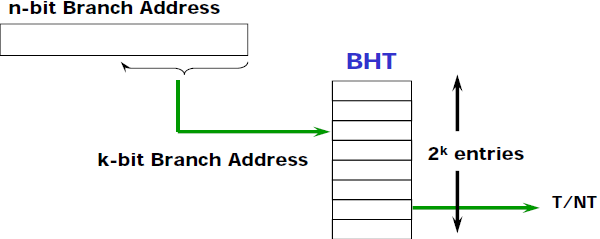
\includegraphics[scale=0.5]{img/historytable.png}
\caption{Esempio di \emph{Branch History Table}}\label{fig:historytable}
\end{figure}
Una predizione errata avviene quando una predizione risulta sbagliata oppure quando un indice è puntato da due differenti salti e la previsione si riferisce all'altro salto, per risolvere questo problema è sufficiente incrementare il numero di righe della BHT o utilizzare una funzione di hash.\\
Nel caso di una BHT ad un solo bit e considerando per esempio un salto di un loop che solitamente è eseguito la BHT sbaglierà predizione due volte, nel caso non sia eseguito e nel caso in cui venga eseguito il salto subito dopo non essere stato eseguito. Per meglio specificare i due casi abbiamo:
\begin{itemize}
\item All'ultima iterazione quando il salto non viene eseguito anche se la predizione indicava il contrario
\item Quando rientriamo nel loop alla fine della prima interazione la nostra predizione indica che dovremmo uscire (ultima interazione del loop precedente) mentre in realtà effettueremo il salto. 
\end{itemize}
Per ovviare a questo problema sfruttiamo una BHT a due bit nella quale sono necessarie due predizioni sbagliate consecutive per cambiare la nostra predizione. Per ogni indice della tabella i due bit sono utilizzati per indicare un dei quattro stati della macchina a stati finita in \figurename\,\ref{fig:bhtfsm}
\begin{figure}[htb]
\centering
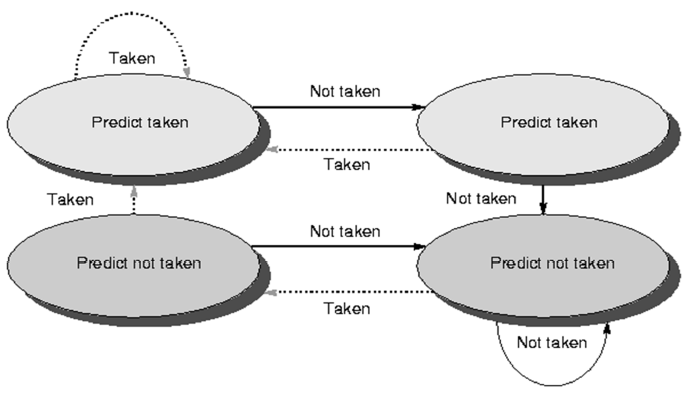
\includegraphics[scale=0.4]{img/bhtfsm.png}
\caption{Macchina a stati finita per una BHT a 2 bit}\label{fig:bhtfsm}
\end{figure}
Tale tecnica si può generalizzare fino ad utilizzare una tabella con \emph{n} bit per ogni record. Il valore che può assumere questo record va da 0 a $2^n-1$; quando il valore del record diventa uguale ad almeno la metà del suo valore massimo ($2^n-1$) la predizione del salto indica che esso deve essere eseguito, altrimenti la predizione sarà che non deve essere eseguito. Nello schema precedente il contatore veniva incrementato quando il salto veniva intrapreso e decrementato quando non veniva intrapreso.
\\ Tuttavia anche se una generalizzazione è possibile gli studi hanno dimostrato che una una tabella a 2 bit fornisce dati più che soddisfacenti. Ad esempio per una architettura IBM \emph{SPEC89} con una BHT con 4K record di 2 bit l'accuratezza nella predizione varia dal $99\%$ all'$82\%$.\\
La BHT a 2 bit utilizza solo i risultati delle esecuzioni precedenti di un singolo salto per predire il risultato di quel salto. L'idea di base però è che il comportamento dei salti recenti è che essi sono correlati con il comportamento di altri salti e perciò la predizione può essere influenzata da tali comportamenti. Un esempio è mostrato in \figurename\,\ref{fig:correletedbranch}
\begin{figure}[htb]
\centering
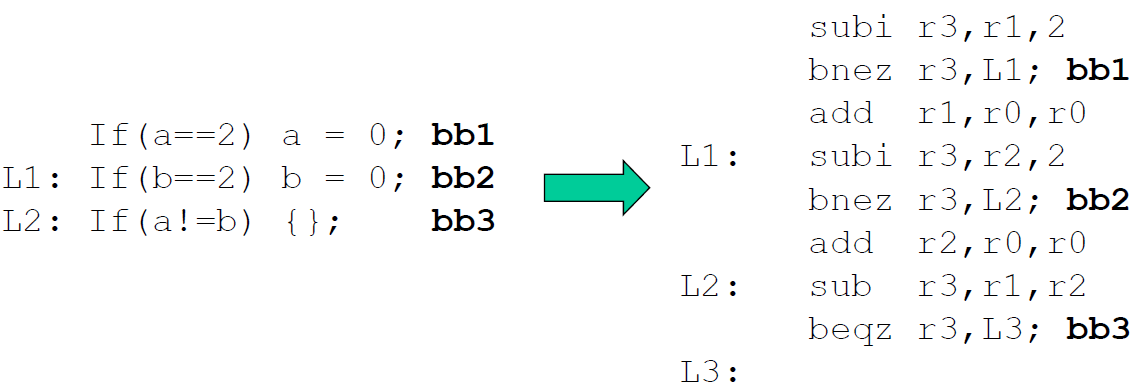
\includegraphics[scale=0.5]{img/correleted.png}
\caption{Esempio di salti correlati}\label{fig:correletedbranch}
\end{figure}
Un predittore che utilizza il comportamento di altri salti per effettuare una predizione è chiamato \textbf{Correlating  Predictors} o anche \textbf{2-Level Predictors}.
Un esempio di un \emph{(1,1) Correlating Predictors} è un predittore ad un bit con un bit di correlazione, ovvero il comportamento dell'ultimo salto è utilizzato per scegliere una coppia di predittori ad un bit come mostrato in \figurename\,\ref{fig:11correlato}.
\begin{figure}
\centering
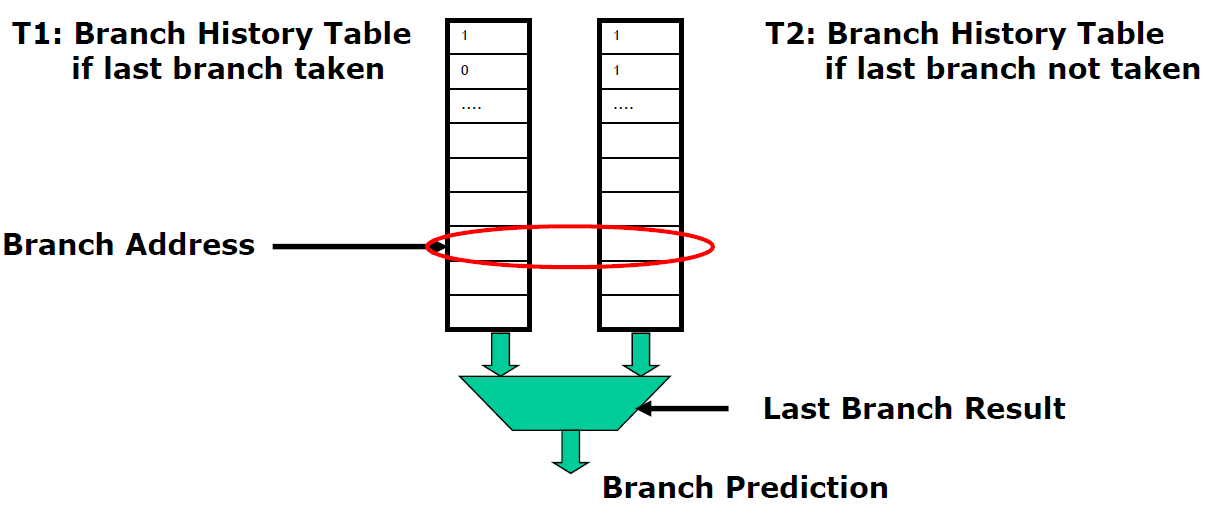
\includegraphics[scale=0.5]{img/11correlato.png}
\caption{Esempio di predittore correlato di tipo (1,1)}\label{fig:11correlato}
\end{figure}
Si registrano le esecuzioni degli ultimi k salti; la predizione si basa sull'esecuzione del salto precedente selezionando la BHT ad un bit appropriata:
\begin{itemize}
\item Una predizione è usata nel caso in cui l'ultimo salto è stato eseguito.
\item L'altra predizione è utilizzata se l'ultimo salto non è stato intrapreso.
\end{itemize}
In generale l'esecuzione dell'ultimo salto non riguarda la stessa istruzione sulla quale si cerca di fare una predizione come normalmente accade nei loop semplici.\\
In generale possiamo costruire un predittore correlato con (m,n) dove \emph{m} indica gli ultimi \emph{m} salti da analizzare selezionando $2^m$ BHT ognuna delle quali è un predittore a \emph{n} bit.
Il branch prediction buffer può essere indicizzato concatenando la parte finale del branch address con gli \emph{m} bit della \emph{global history}.
Un esempio di un predittore correlato è un predittore (2,2) dove si hanno quattro BHT a 2 bit tra i quali scegliere e si usano 2 bit dalla global history per selezionare quale utilizzare come mostrato in \figurename\,\ref{fig:22correlato}
\begin{figure}[htb]
\centering
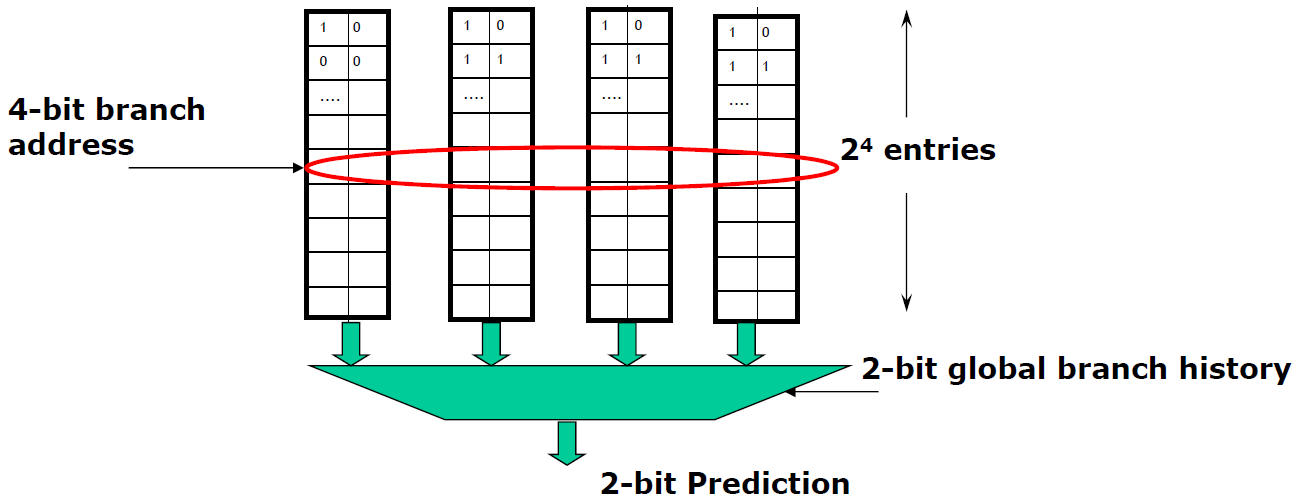
\includegraphics[scale=0.5]{img/22correlato.png}
\caption{Esempio di predittore correlato (2,2)}\label{fig:22correlato}
\end{figure}
Un predittore a due bit non correlato non è altro che un predittore correlato con i valori (0,2); a questo punto possiamo confrontare le performance nel caso di un predittore semplice a 2 bit con una tabella di 4K entità e un predittore correlato (2,2) con tabelle di 1K entità. Come vediamo dal grafico in \figurename\,\ref{fig:performance}
Il predittore correlato è, in molti casi più efficace di un predittore semplice mentre nei casi peggiori ne eguaglia le performance.
\begin{figure}[htb]
\centering
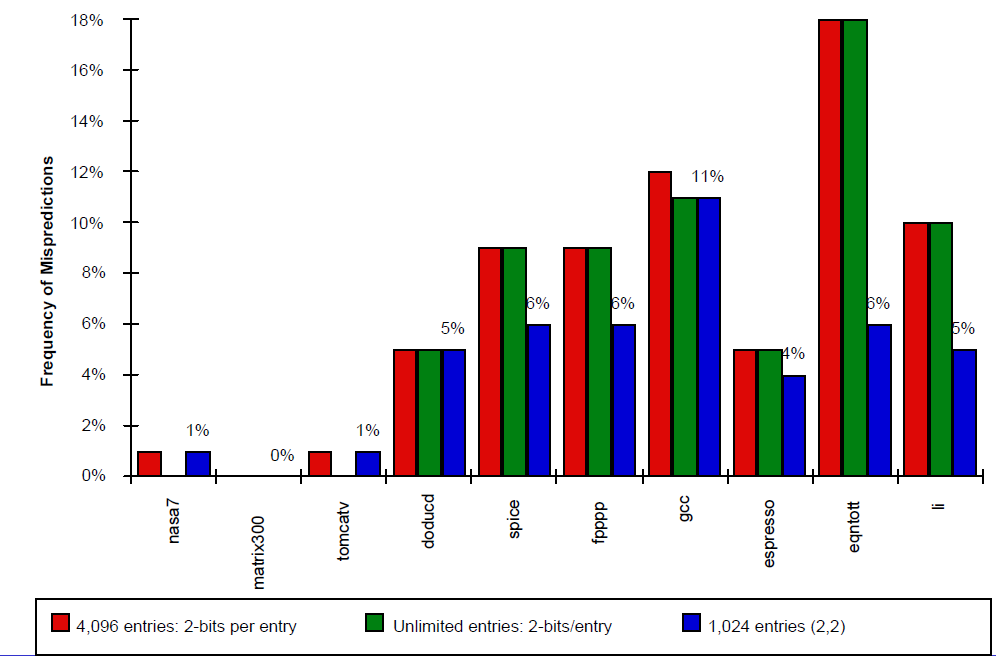
\includegraphics[scale=0.5]{img/performance.png}
\caption{Comparazione delle performance per predittore non correlato e predittore corellato}\label{fig:performance}
\end{figure}
Un altra tecnica di predizione dinamica è quella del \textbf{Predittore di salto adattativo a due livelli} (\emph{Two-Level Adaptative Branch Predictors}) nel quale un primo livello di storia viene memorizzato in uno shift register a \emph{k} bit chiamato \textbf{Branch History Register (BHR)} il quale memorizza i risultati degli ultimi k salti. Il secondo livello di storicizzazione è memorizzato in una tabella con record di due bit chiamata \textbf{Pattern History Table (PHT)} per indicare la predizione.
La BHR è utilizzata per indicizzare la PHT e selezionare i due bit da utilizzare; per selezionare quale dei due bit utilizzare si utilizza lo stesso principio utilizzato per i predittori a due bit semplici.
\begin{figure}[htb]
\centering
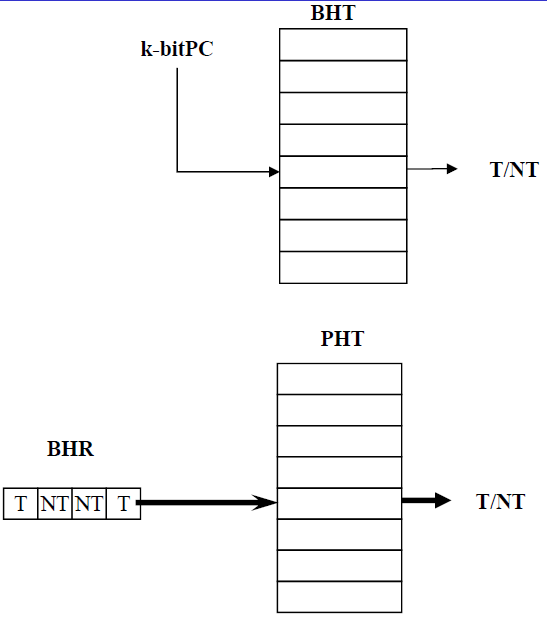
\includegraphics[scale=0.5]{img/gapred.png}
\caption{Esempio di predittore adattativo}\label{fig:gapred}
\end{figure}
Un evoluzione di questo predittore è il \textbf{predittore GShare} dove le informazioni dell'indirizzo locali vengono correlate con quelle globali tramite un'operazione di XOR.
\begin{figure}[htb]
\centering
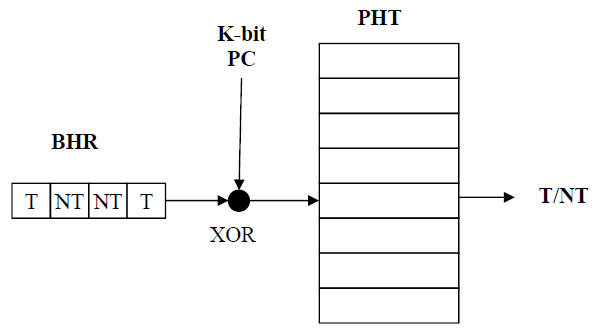
\includegraphics[scale=0.5]{img/gshare.png}
\caption{Esempio di predittore GShare}\label{fig:gshare}
\end{figure}
Un ultimo elemento importante nella predizione dinamica è il \textbf{Branch Target Buffer} la quale è una cache nella quale vengono memorizzate l'indirizzo di destinazione del salto per le istruzioni dopo il salto. Accediamo al BTB nello stage IF utilizzando l'indirizzo dell'istruzione da prelevare per indicizzare la cache. Un possibile esempio di record è mostrato in \figurename\,\ref{fig:btbrecord}.
\begin{figure}[htb]
\centering
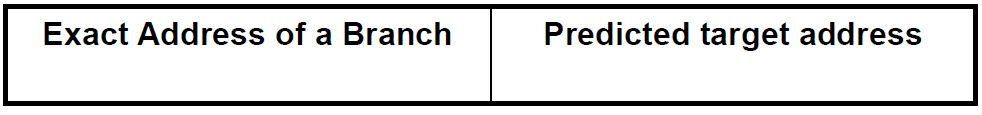
\includegraphics[scale=0.5]{img/btbrecord.png}
\caption{Esempio di record di un Branch Target Buffer}\label{fig:btbrecord}
\end{figure}
L'indirizzo di destinazione  del salto è espresso sempre in modo relativo al PC.
La struttura del BTB è mostrata in \figurename\,\ref{fig:btbstrut}; in tale buffer dobbiamo memorizzare solo gli indirizzi per quei salti che vengono eseguiti.
\begin{figure}[htb]
\centering
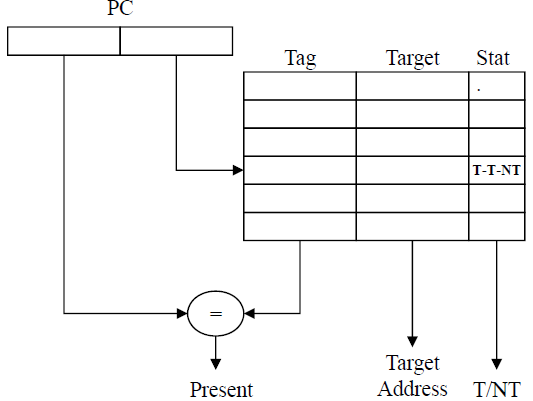
\includegraphics[scale=0.5]{img/btbstrut.png}
\caption{Struttura di un Branch Target Buffer}\label{fig:btbstrut}
\end{figure}
\subsection{Speculazione}
Senza tecniche di predizione di salto il parallelismo risulta molto limitato e si riduce all'analisi dei \textbf{basic block} ovvero a pezzi di codice nei quali non entrano o escono dei salti. Tuttavia possiamo azzardare alcune supposizioni di parallelismo tra diversi blocchi base effettuando delle speculazioni. Tramite le speculazioni possiamo recuperare ed eseguire le istruzioni come se le nostre predizioni siano corrette gestendo in seguito il caso in cui non siano corrette. Tale speculazione può essere supportata sia dal compilatore che dall'hardware.